\documentclass[11pt,a4paper]{article}
\author{TalentSprint}
\date{}
\usepackage{fancyhdr}
\usepackage{latexsym}
\usepackage{soul}
\usepackage{verbatim}
\usepackage{graphicx}
\usepackage{array}
\usepackage{enumerate}
\usepackage{multicol}
\usepackage{xcolor}
\usepackage[tikz]{bclogo}
\usepackage{textcomp}
\usepackage{latexsym}
\usepackage{seqsplit} 
\usepackage{setspace}
\usepackage{listings}
\lstset{language=html,numbers=left,numberstyle=\tiny,numbersep=10pt,showstringspaces=false}
\usepackage{fancyhdr}
\headheight=14pt
\lhead{\nouppercase{}}
\rhead{\nouppercase{\leftmark}}

\graphicspath{{../Images/}}

%\pagestyle{fancy}

%========================================================================

% Lengths and widths
\addtolength{\textwidth}{2.5cm}
\addtolength{\hoffset}{0cm}
\setlength{\headsep}{-12pt} % Reduce space between header and content
\setlength{\headheight}{85pt} % If less, LaTeX automatically increases it
\renewcommand{\footrulewidth}{2pt} % Remove footer line
\renewcommand{\headrulewidth}{1pt} % Remove header line
\renewcommand{\seqinsert}{\ifmmode\allowbreak\else\-\fi} % Hyphens in seqsplit
% This two commands together give roughly
% the right line height in the tables
\renewcommand{\arraystretch}{1.3}
\onehalfspacing



% Commands
\newcommand{\SetRowColor}[1]{\noalign{\gdef\RowColorName{#1}}\rowcolor{\RowColorName}} % Shortcut for row colour
\newcommand{\mymulticolumn}[3]{\multicolumn{#1}{>{\columncolor{white}}#2}{#3}} % For coloured multi-cols
\newcolumntype{x}[1]{>{\raggedright}p{#1}} % New column types for ragged-right paragraph columns
\newcommand{\tn}{\tabularnewline} % Required as custom column type in use

% Font and Colours
\definecolor{HeadBackground}{HTML}{333333}
\definecolor{FootBackground}{HTML}{666666}
\definecolor{TextColor}{HTML}{333333}
\definecolor{DarkBackground}{HTML}{6B8E23} %{FD1AA8}
\definecolor{LightBackground}{HTML}{E8FED8} %D3FDC8
\definecolor{tit}{HTML}{FF6600}
\renewcommand{\familydefault}{\sfdefault}
\color{TextColor}
 \headsep = 25pt
% Header and Footer
\pagestyle{fancy}
\usepackage[headheight=110pt]{geometry}
\fancyhf{}% Clear header/footer

\fancyhead[r]{
\includegraphics[width = 4cm, height = 2cm]{TS-Logo.png}\hspace{0cm}}

%=================================TITLE=====================================
\fancyhead[l]{{\bf{\textcolor{tit}{\textrm{\large{Getting Started With Java}}}}}}
%===========================================================================

\renewcommand{\headrulewidth}{0.4pt}% Default \headrulewidth is 0.4pt
\renewcommand{\footrulewidth}{0.4pt}% Default \footrulewidth is 0pt

\rfoot{Page \thepage}
\lfoot{COPYRIGHT \textcopyright TALENTSPRINT, 2015. ALL RIGHTS RESERVED.}


\begin{document}

\section*{Java Basics}
\subsection*{History of Java}
The original name of Java was Oak, and it was developed as a part of the Green project at Sun Microsystems. Java was conceived by James Gosling, Patrick Naughton, Chris Warth, Ed Frank, and Mike Sheridon at Sun Microsystems in 1991.

The design objectives of the team were to come up with a language that:
\begin{itemize}
\item ensured security
\item ensured reliability
\item would be platform independent -- one that would function seamlessly, regardless of the CPU
\end{itemize}
The World Wide Web (WWW), by nature, had requirements such as reliability, security, and architecture independence, which were in line with the design goals of Java. Sun formally announced the Java language in SunWorld Conference in 1995.
On January 27, 2010, Sun was acquired by Oracle Corporation.

Oracle has three major Java products: 
\begin{enumerate}
 \item Java Platform Standard Edition (\textbf{Java SE}) for desktop application development.
 \item Java Platform Enterprise Edition (\textbf{Java EE}) for enterprise application development.
 \item Java Platform Micro Edition (\textbf{Java ME}) for mobile application development.
\end{enumerate}
\begin{comment}
\begin{bclogo}[couleur=blue!5, arrondi=0.3]{Note:}
\begin{description}
 \item [Java SE] - Java Platform Standard Edition
 \item [Java EE] - Java Platform Enterprise Edition
 \item [Java ME] - Java Platform Micro Edition
\end{description}

\end{bclogo}
\end{comment}
\subsection*{Java Major Versions}
\begin{multicols}{2}
\begin{itemize}
    \item JDK Alpha and Beta -- 1995
    \item JDK 1.0 -- January 23, 1996
    \item JDK 1.1 -- February 19, 1997
    \item J2SE 1.2 -- December 8, 1998
    \item J2SE 1.3 -- May 8, 2000
    \end{itemize}
    \begin{itemize}
    \item J2SE 1.4 -- February 6, 2002
    \item J2SE 5.0 -- September 30, 2004
    \item Java SE 6 -- December 11, 2006
    \item Java SE 7 -- July 28, 2011
    \item Java SE 8 -- March 18, 2014 
\end{itemize}
\end{multicols}
\subsection*{Java Technology}
The word Java refers to many things.
\begin{itemize}
\item Java is a programming language.
\item Java is a development environment that provides tools such as compiler, interpreter, documentation generator, and so on.
\item Java is an application environment to run standalone programs that run on any machine where the Java Runtime Environment (JRE) is installed.
\item Java is a deployment environment that supplies Java SE Development Kit with complete set of Application Programming Interface (APIs) as packages.
\item Java provides an easy-to-use language by avoiding pitfalls of other languages, such as pointer arithmetic and memory management, which affect the robustness of the code.
\end{itemize}
\subsection*{Features of Java}
\begin{enumerate}
\item Simple
\begin{itemize}
\item Java is Easy to write and more readable and eye catching.
\item Java has a concise, cohesive set of features that makes it easy to learn and use.
\item Most of the concepts are drew from C / C++ thus making Java learning simpler.
\end{itemize}

\item Object Oriented
\begin{itemize}
 \item Object-oriented means organizing software as a combination of different types of objects that incorporates both data and behaviour.
 \item Object-oriented programming(OOPs) is a methodology that simplify software development and maintenance by providing some rules.
 \item Basic concepts of OOPs are:
 \begin{itemize}
   \item Object
   \item Class
   \item Inheritance
   \item Polymorphism
   \item Abstraction
  \item Encapsulation
 \end{itemize}
\end{itemize}

\item Portable
\begin{itemize}
\item The portability actually comes from architecture-neutrality. In C/C++, source code may run slightly differently on different hardware platforms because of how these platforms implement arithmetic operations. In Java, it has been simplified.

Unlike C/C++, in Java the size of the primitive data types are machine independent. For example, an int in Java is always a 32-bit integer, and float is always a 32-bit IEEE 754 floating point number. These consistencies make Java programs portable among different platforms such as Windows, Linux and Mac OS.
\end{itemize}

\item Platform Independent
\begin{itemize}
 \item Java source code (.java file) is compiled by the Java compiler (javac) and converted into bytecode (.class file).
 \item Java bytecode can be executed on multiple platforms e.g. Windows, Linux and Mac OS, that has Java Virtual Machine (JVM).
 \item JVM converts the bytecode to machine specific code. Thus JVM makes Java as platform independent.
\vfill{\ }
   \begin{figure}[H]
 \begin{center}
 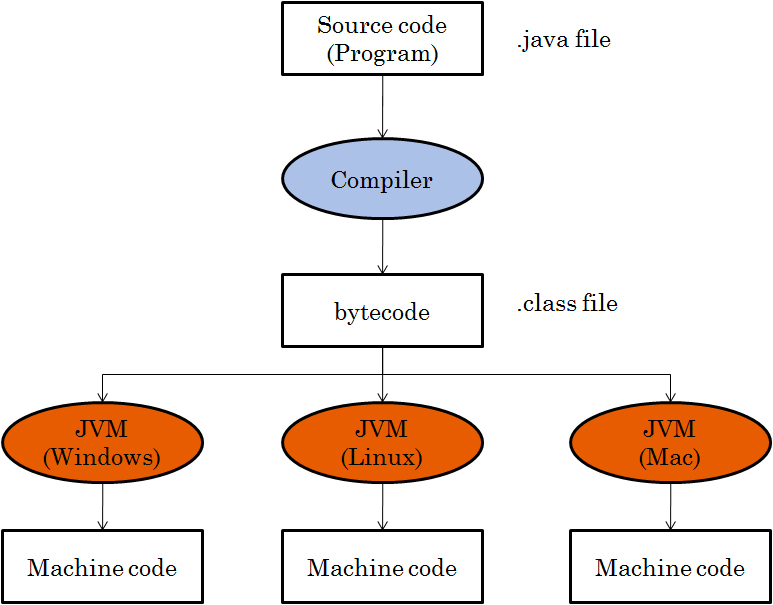
\includegraphics[scale=0.3]{platform.jpg}
\caption{Platform Independency}
 \end{center}
 \end{figure}
 \end{itemize}

 \item Robust
\begin{itemize}
\item Reliable - that the code works as desired in normal circumstances for specified periods of time.
\item Robustness - the code responding appropriately in abnormal circumstances.
\item Strong Error handling mechanism: Lot of checks are done at the compilation itself. More checks are performed at runtime system to make sure that code does not malfunction.
\item Automatic garbage collection

\end{itemize}
\item Multithreaded
\begin{itemize}
\item At the OS level, smallest unit of work that can be scheduled, is a thread.
\item Thread is a sequence of execution of code.
\item A process consists of one or more threads.
\item Multiple threads in the same program share same resources.
\item Unlike a multiple process, multiple threads in a process share same memory location. That is why threads are sometimes called Light weight process.
\item Java Standard API has rich set of classes that allows us to work with multiple threads simultaneously
\end{itemize}

\item Dynamic and Extensible

\begin{itemize}
\item Java has Dynamic and Extensible means with the help of OOPS Java provides inheritance and with the help of inheritance we reuse the code that is pre-defined and also uses all the built in functions of Java and Classes
\end{itemize}
 
\item Security
\begin{itemize}
 \item With Java's secure feature it enables to develop virus-free, tamper-free systems. Authentication techniques are based on public-key encryption.
\end{itemize}

\item High performance
\begin{itemize}
 \item With the use of Just-In-Time (JIT) compilers, Java enables high performance.
\end{itemize}

\end{enumerate}
\section*{First Java Program}

Now let us write a program which displays ``Hello World'' on console.

Follow the steps below:
\begin{description}
\item [Step 1]
 Open a terminal and type below command to create a file.
\begin{lstlisting}[numbers=none]
$ vim Welcome.java
\end{lstlisting}
\item [Step 2]
 Type the below code in the file.
\lstinputlisting{../Code/Welcome.java}
\item [Step 3] Save and quit from the file 
   Press \textbf{Esc :wq}
\item [Step 4] Type the below command in terminal to compile the source code 
\begin{lstlisting}[numbers=none]
$ javac Welcome.java
\end{lstlisting}

 \emph{Note: If the source code is compiled without any errors, it creates a \texttt{.class} file (\texttt{Welcome.class})}
 \item [Step 5] Type the below command to execute the file.

\begin{lstlisting}[numbers=none]
$ java Welcome
\end{lstlisting}

Once the execution is done, you can see the output as shown below:
 \begin{figure}[H]
 \begin{center}
   
\includegraphics[scale=0.5]{Welcome.png}
 \end{center}
 \end{figure}
\end{description}

\subsubsection*{Analysis of the program}

As shown in above code, following is the most basic form of a class definition
\begin{lstlisting}[numbers=none]
 class Welcome {
    . . .
 }
\end{lstlisting}

The keyword \lstinline!class! begins the class definition for a class named ``Welcome'', and the code for each class appears between the opening and closing braces. Every Java application begins with a class definition.
\begin{lstlisting}[numbers=none]
 public static void main(String[] args) {
    . . .
 }
\end{lstlisting}

Every Java application must contain a main method.

The modifiers \lstinline!public! and \lstinline!static! can be written in either order (public static or static public), but the convention is to use public static as shown above. You can name the argument anything you want, but most programmers choose ``args'' or ``argv''.

The main method is similar to the main function in C and C++, it's the entry point for your application and will subsequently invoke all the other methods required by your program.

The main method accepts a single argument, an array of elements of type String.

\begin{lstlisting}[numbers=none]
 System.out.println(``Hello world'');
\end{lstlisting}

Uses the \lstinline!System! class from the core library to print the ``Hello World'' message to standard output.
\vfill{\ }
\begin{figure}[H]
 \begin{center}
   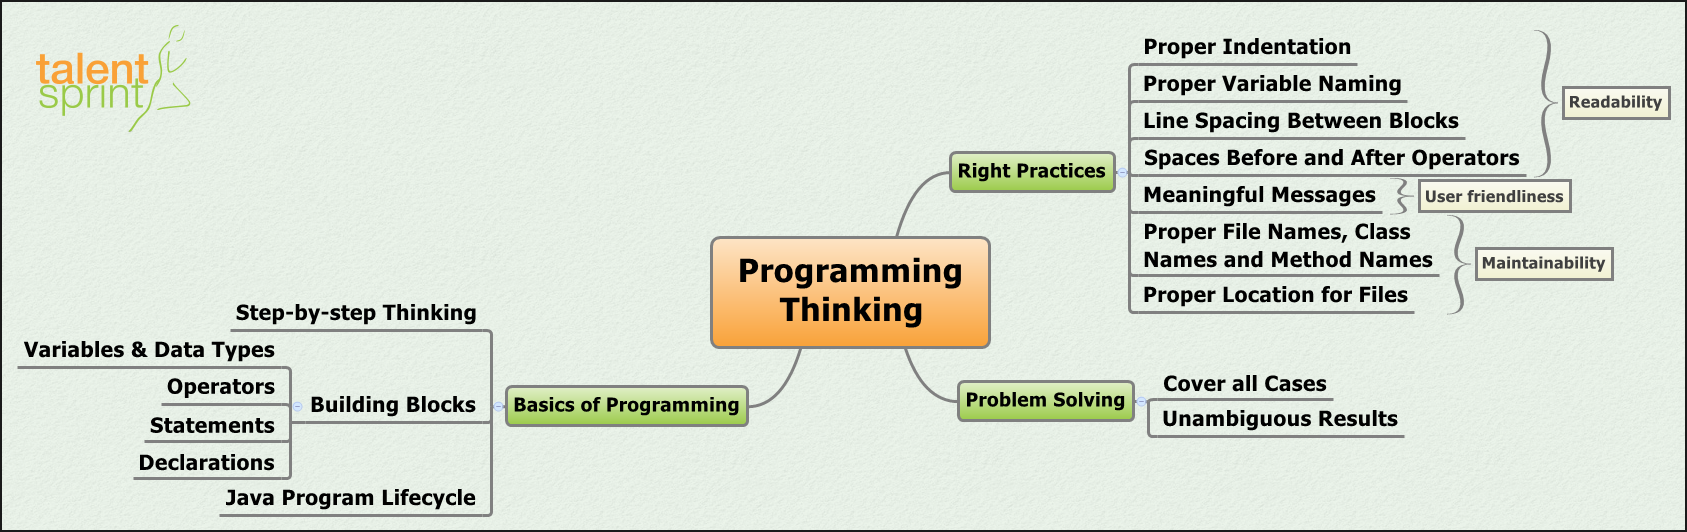
\includegraphics[angle=90,height=19cm, width=12cm]{ProgrammingThinking.png}
 \end{center}
 \end{figure}
\section*{Language Fundamentals}
\subsection*{Comments}
Comments are used to document and explain your codes and program logic. Comments are not programming statements and are ignored by the compiler, but they VERY IMPORTANT for providing documentation and explanation to understand the program.

There are two kinds of comments in Java:
\begin{description}
\item [Single-line Comment] begins with // and lasts till the end of the current line.
\item [Multi-line Comment] begins with a /* and ends with a */, and can span several lines.
\end{description}
Use comments liberally to explain and document your codes. During program development, instead of deleting a chunk of statements irrevocably, you could comment-out these statements so that you could get them back later, if needed.
\subsection*{Keywords}
Keywords are predefined identifiers reserved by Java for a specific purpose. You cannot use keywords as names for your variables, classes and methods.

\begin{multicols}{4}
 \begin{description}
  \item abstract
  \item assert***
  \item boolean
  \item break
  \item byte
  \item case
  \item catch
  \item char
  \item class
  \item const*
  \item continue
  \item default
  \item do
  \end{description}
   
 \begin{description}
  \item double  
  \item else
  \item enum****
  \item extends 
  \item final
  \item finally
  \item float
  \item for
  \item goto*
  \item if
  \item implements
  \item import
  \item instanceof
  \end{description}
   
 \begin{description}
  \item int
  \item interface
  \item long
  \item native
  \item new
  \item package
  \item private
  \item protected 
  \item public
  \item return
  \item short
  \item static
  \item strictfp**
  \end{description}
   
 \begin{description}  
  \item super
  \item switch
  \item synchronized
  \item this
  \item throw
  \item throws
  \item transient
  \item try
  \item void
  \item volatile
  \item while
  \item
  \item
  \end{description}
   \end{multicols}
  
   \emph{Note : \\ 1. * not used, ** added in 1.2, *** added in 1.4, **** added in 5.0 \\
   2. The symbolic constants \lstinline!null!, \lstinline!true! and \lstinline!false! are not keywords. They cannot be used for any other purpose.}

\subsection*{Data Types}
Data type specifies the size and type of values that can be stored in an identifier. The Java programming language is statically-typed, which means that all variables must first be declared before they can be used. This involves stating the variable's type and name, as you have learnt in C Programming Language.

Data types in Java are classified into two types:
\begin{description}
\item [Primitive data types] are predefined by the language and is named by a reserved keyword. Primitive values do not share state with other primitive values. The eight primitive data types supported by the Java programming language are:
\begin{description}
\item [byte] The byte data type is an 8-bit signed two's complement integer. It has a minimum value of -128 and a maximum value of 127 (inclusive). The byte data type can be useful for saving memory in large arrays.
\item [short] The short data type is a 16-bit signed two's complement integer. It has a minimum value of -32,768 and a maximum value of 32,767 (inclusive).
\item [int] The int data type is a 32-bit signed two's complement integer, which has a minimum value is - 2,147,483,648 and a maximum value - 2,147,483,647. 
\item [long] The long data type is a 64-bit two's complement integer. The signed long has a minimum value is  -9,223,372,036,854,775,808 and a maximum value  -9,223,372,036,854,775,807.
\item [float] The float data type is a single-precision 32-bit IEEE 754 floating point. Use a float (instead of double) if you need to save memory in large arrays of floating point numbers. 
\item [double] The double data type is a double-precision 64-bit IEEE 754 floating point. For decimal values, this data type is generally the default choice. 
\item [boolean] The boolean data type has only two possible values: \lstinline!true! and \lstinline!false!. Use this data type for simple flags that track true/false conditions. This data type represents one bit of information.
\item [char] The char data type is a single 16-bit Unicode character. It has a minimum value of `\textbackslash u0000' (or 0) and a maximum value of `\textbackslash uffff' (or 65,535 inclusive).
\end{description}
\item [Non-primitive data types] are not defined by the programming language, but are instead created by the programmer. They are sometimes called ``reference variables'' or ``object references'', since they reference a memory location, which stores the data.

\end{description}

\subsection*{Literals}
A literal, or literal constant, is a specific constant value or raw data, such as 123, -456, 3.14, `a', ``Hello'', that is used in the program source. It can be assigned directly to a variable, or used as part of an expression. They are called literals because they literally and explicitly identify their values. We call it literal to distinguish it from a variable.
\begin{description}
\item [Integer Literals]
An integer literal is of type \lstinline!long! if it ends with the letter `L'or `l', otherwise it is of type \lstinline!int!. It is recommended that you use the upper case letter `L' because the lower case letter `l' is hard to distinguish from the digit 1.

Values of the integral types \lstinline!byte, short, int,! and \lstinline!long! can be created from \lstinline!int! literals. Values of type \lstinline!long! that exceed the range of \lstinline!int! can be created from \lstinline!long! literals. Integer literals can be expressed by these number systems:
\begin{description}
\item [Decimal] - Base 10, whose digits consists of the numbers 0 through 9, this is the number system you use every day
\item [Hexadecimal] - Base 16, whose digits consist of the numbers 0 through 9 and the letters A through F
\item [Binary] - Base 2, whose digits consists of the numbers 0 and 1 (you can create binary literals in Java SE 7 and later)
\end{description}
For general-purpose programming, the decimal system is likely to be the only number system you will ever use. However, if you need to use another number system, the following example shows the correct syntax. The prefix \texttt{0x} indicates hexadecimal and \texttt{0b} indicates binary:
\begin{lstlisting}[numbers=none]
// The number 26, in decimal
int decVal = 26;
//  The number 26, in hexadecimal
int hexVal = 0x1a;
// The number 26, in binary
int binVal = 0b11010;
\end{lstlisting}
\item [Floating-Point Literals]
A number with a decimal point, such as 55.66 and -33.44, is treated as a double, by default. You can also express them in scientific notation, e.g., 1.2e34, -5.5E-6, where e or E denotes the exponent in power of 10. You could precede the fractional part or exponent with a plus (+) or minus (-) sign. Exponent values are restricted to integer. There should be no space or other characters in the number.

You can optionally use suffix `d' or `D' to denote double literals.

You MUST use a suffix of `f' or `F' for float literals, e.g., -1.2345F. For example,
\begin{lstlisting}[numbers=none]
float average = 55.66;      // Error! RHS is a double. Need suffix 'f' for float.
float average = 55.66f;
\end{lstlisting}
\item [Character Literals]
A printable char literal is written by enclosing the character with a pair of single quotes, e.g., `z', `\$', and `9'.
\item [String Literals]
A String literal is composed of zero or more characters surrounded by a pair of double quotes, e.g., ``Hello, world!'', ``The sum is ''. For example,
\begin{lstlisting}[numbers=none]
String directionMsg = ``Turn Right'';
String greetingMsg = ``Hello'';
String statusMsg = ``'';    // empty string
\end{lstlisting}
\end{description}
\subsection*{Type Casting}
Type Casting is the mapping type of an object to another. Casting between primitive types enables you to convert the value of one data from one type to another primitive type, commonly occurs between numeric types. Boolean data type can't be converted to other types.

Types of Casting:
\begin{enumerate}
\item Implicit Casting
\item Explicit Casting
\end{enumerate}
\begin{description}
\item [Implicit Casting] means that a value of one type is changed to a value of another type without any special directive from the programmer. A \lstinline!char! can be implicitly converted to an \lstinline!int!, a \lstinline!long!, a \lstinline!float!, or a \lstinline!double!. 

Suppose you want to store a value of \lstinline!int! to \lstinline!double!.
\begin{verbatim}
int numInt = 10;
double numDouble = numInt; //implicit cast
\end{verbatim}
\item [Explicit Casting] is done via casting. The name of the type to which you want a value converted is given, in parentheses, in front of the value. When you convert a data that has a larger type to a smaller type, you must use explicit casting. For example, the following code casts a value of type \lstinline!double! to a value of type \lstinline!int!.
\begin{verbatim}
double valDouble = 10.12;
int valInt = (int)valDouble;
\end{verbatim}
\end{description}

\subsection*{Operators}
An operator is a symbol that operates on one or more operands to produce a result. There are many operators available in Java language.
\begin{description}
\item [Arithmetic Operators] $\Longrightarrow$ +, -, *, \%, /
\item [Relational Operators] $\Longrightarrow$  $>$, $<$, $>=$, $<=$, !=, ==
\item [Assignment Operator] $\Longrightarrow$  =
\item [Unary Operators]  $\Longrightarrow$ ++, - -
\item [LogicalOperators] $\Longrightarrow$ \&\&, $\parallel$, ! 
\end{description}

\section*{Control Statements}
The control statements are used to control the flow of execution of the program. The execution order depends on the supplied data values and the conditional logic.

Types of control statements:

\begin{enumerate}
 \item	Conditional Statements
 \begin{enumerate}
  \item if
  \item if else
  \item else if
  \item nested if
  \item switch
 \end{enumerate}
 \item	Looping Statements
 \begin{enumerate}
  \item while
  \item for
  \item do while
 \end{enumerate}
\end{enumerate}

\subsection*{Conditional Statements}
\begin{description}
\item [if] statement will execute a single statement or a block of statements, when the given boolean expression is \lstinline!true! and if it is \lstinline!false! then it skips if block and executed the statements after the if block.
\begin{lstlisting}[numbers=none]
    if (boolean_expression) {
        statement(s);
    }

\end{lstlisting}

\item [if-else] statement provides a secondary path of execution when an \lstinline!if! statement evaluates to \lstinline!false!.
\begin{lstlisting}[numbers=none]
    if (boolean_expression) {
        A-statement(s);
    } else {
        B-statement(s);
    }
\end{lstlisting} 

\item [if-else if] statement can be followed by an optional \lstinline!else if...else! statement, which is very useful to test various conditions using single \lstinline!if...else if! statement.

\begin{lstlisting}[numbers=none]
    if (boolean_expression1) {
        A-statement(s);
    } else if (boolean_expression2) {
        B-statement(s);
    } else if (boolean_expression3) {
        C-statement(s);
    } else {
        D-statement(s);
    }

\end{lstlisting} 
\item [nested-if] statement is an \lstinline!if-else! statement with another \lstinline!if! statement as the \lstinline!if! body or the \lstinline!else! body.

\begin{lstlisting}[numbers=none]
    if (boolean_expression1) {
        if (boolean_expression2) {
            A-statement(s);
        } else {
            B-statement(s);
        }
    } else {
        C- statement(s);
    }
   
\end{lstlisting}

\item [switch] statement can have a number of possible execution paths. A \lstinline!switch! works with the \lstinline!byte!, \lstinline!short!, \lstinline!char!, and \lstinline!int! primitive data types. The expression in switch can be a \lstinline!String! (Introduced in Java 1.7) type.

\begin{lstlisting}[numbers=none]
    switch (expression) {
        case value1:
            statement(s);
            break;
        case value2:
            statement(s);
            break;
        case valueN:
            statement(s);
            break;
        default:
            statement(s);
    }   
\end{lstlisting}
\end{description}
\vfill{\ }
\begin{figure}[H]
 \begin{center}
   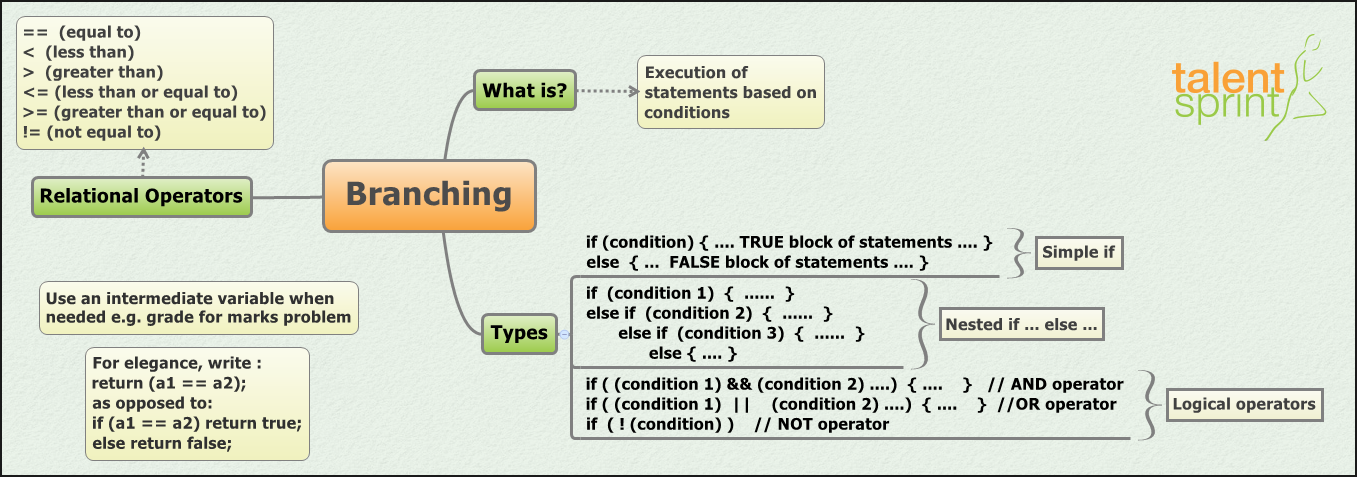
\includegraphics[angle=90,height=20cm, width=13cm]{Branching.png}
   
 \end{center}
 \end{figure}
\subsection*{Looping Statements}
\begin{description}
\item [While] statement continually executes a block of statement(s) until the given boolean expression is \lstinline!false!.
\begin{lstlisting}[numbers=none]
    while (boolean_expression) {
        statement(s);
    }
\end{lstlisting}

\item [do-while ] is similar to \lstinline!while!, but it evaluates the boolean expression after executing the block of statement(s).
\begin{lstlisting}[numbers=none]
    do {
        statement(s);
    } while (boolean_expression);
\end{lstlisting}

\item [for ] loop controls a sequence of repetitions. A basic \lstinline!for! structure has three parts: \emph{init}, \emph{test}, and \emph{update}. Each part must be separated by a semicolon (;). The loop continues until the test evaluates to \lstinline!false!. 
\begin{lstlisting}[numbers=none]
    for (initialization; condition; increment/decrement) {
        statement(s);
    } 
\end{lstlisting}

\end{description}
\vfill{\ }
\begin{figure}[H]
 \begin{center}
   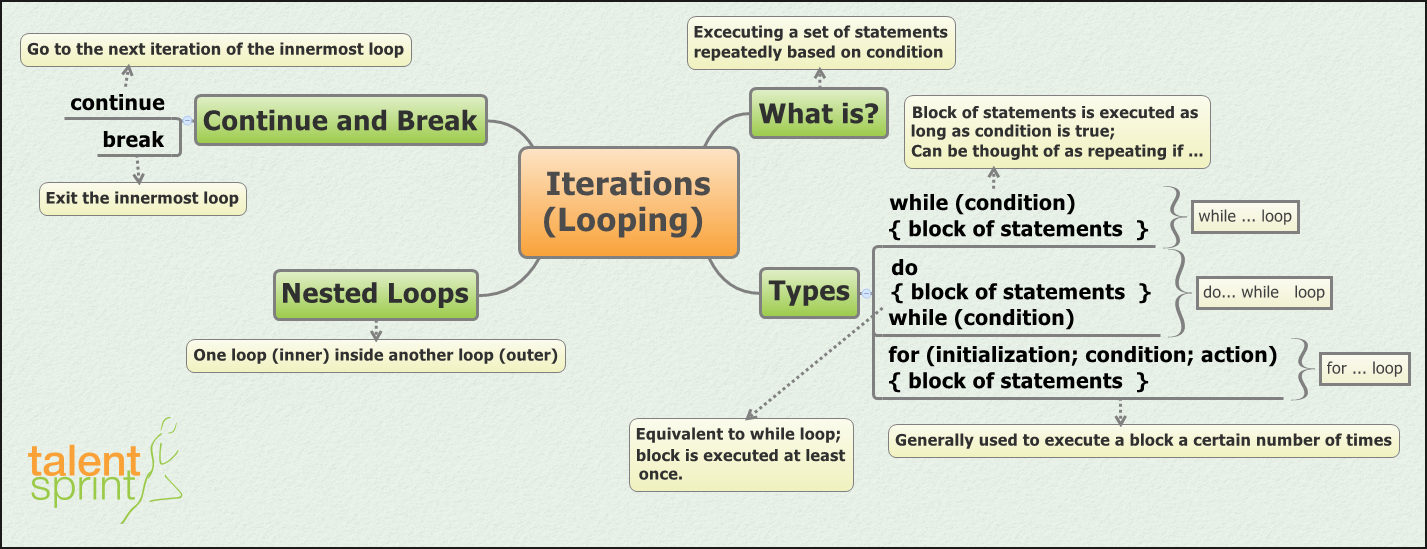
\includegraphics[angle=90,height=20cm, width=13cm]{WhileLoops.png}
 \end{center}
 \end{figure}
\section*{Arrays}
\begin{figure}[H]
 \begin{center}
   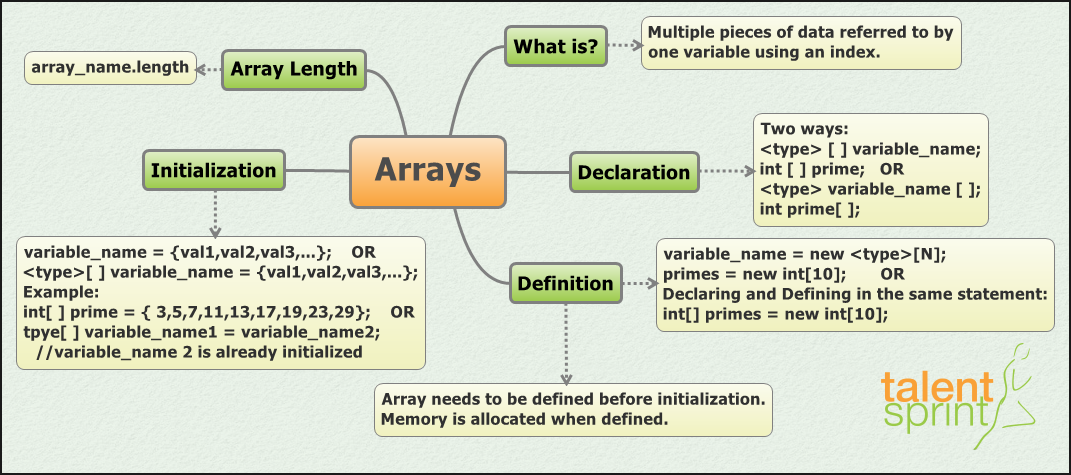
\includegraphics[angle=90,height=20cm, width=13cm]{Arrays.png}
  
 \end{center}
 \end{figure}
Array is a collection of similar type of data. An array is an indexed collection of fixed number of homogeneous data elements. The length of an array is established when the array is created. After creation, its length is fixed.

\subsection*{Creating Arrays} 
An array can be declared by specifying the type of the elements and the number of elements you want to store. Every array in a java is an object, Hence we can create an array by using \lstinline!new! keyword. When an array is constructed via the \lstinline!new! operator, all the elements are initialized to their default values.

An array can be created in any of the two ways:

\lstinline!int[] marks = new int[10];!

\lstinline!int marks[] = new int[10];!

\subsection*{Types of Arrays}
\begin{description}
\item [One-Dimensional-Array] is used to store the data in a row or column wise. if you want to store the roll numbers of 20 students, we can use one-dimensional array.

\lstinline!int[] rollNos = new int[20];!

The above code will create an array named ``rollNos'' of size 20 and initializes the element values to 0.

\item [Two-Dimensional-Array] is used to store data in row and column based index (also known as matrix form). if you want to store roll Numbers and totalMarks secured by 20 students we can use two-dimensional array.

\lstinline!int[][] studMarks = new int[20][2];!

The above code will creat an array named ``studMarks'' of size 20 X 2 and initializes the element values to 0.

\item [Jagged array] contains group of arrays within it. It means we can create an array in Java such that other arrays can become its elements. This is a unique feature in Java. A jagged array can store single dimensional array or multi dimensional arrays and also it can store arrays of any size. Jagged arrays are also called as \lstinline!`irregular multidimensional arrays'!. Jagged arrays are useful when dealing with a group of arrays of different sizes.

To create a jagged array that can store two 1D arrays, we can write as:
\lstinline!int x[][] = new int[2][];!

Here, x is the jagged array with size 2. So, its elements will be x[0] and x[1]. Observe last pair of empty square braces in the expression: new int[2][]. This last pair of braces represents 1D array. So, x[0] and x[1] can store two 1D arrays. Now let us allot memory for x[0] and x[1] so that they can store two 1D arrays of different sizes, as:

\begin{lstlisting}[numbers=none]
x[0] = new int[2];
x[1] = new int[3];
\end{lstlisting} 

So, the first array is represented by x[0] and can have 2 elements which can be referenced as

\lstinline!x[0][0], x[0][1];!

Similarly, the second array which is represented by x[1] can have 3 elements

\lstinline!x[1][0], x[1][1], x[1][2]!

In the same way, we can also cretae a jagged array that contain 2D arrays. For example,

\lstinline!double arr[][][] = new double[3][][];!

Here, arr represents a jagged array with size 3. Observe the last two pairs of empty braces. They represents 2D arrays. So, the jagged array can store 3 other 2 dimensional arrays. The elemets arr[0], arr[1] and arr[2] represent them as

\begin{lstlisting}[numbers=none]
arr[0] = new double[2][3];
arr[1] = new double[2][2];
arr[2] = new double[3][2];
\end{lstlisting}

The first 2D array can have  2 rows and 3 columns. Its elements can be referenced starting from arr[0][0][0] to arr[0][1][2]. The second 2D array can have 2 rows and 2 columns and its elemnts can be referenced from arr[1][0][0] to arr[1][1][1]. The third 2D array can have 3 rows and 2 columns and its elements can vary from arr[2][0][0] to arr[2][2][1].

\begin{description}
\item[Example] Program to demonstrate Jagged arrays.
\lstinputlisting{../Code/JaggedArrayExample.java}
\end{description}
\end{description}

\section*{Command Line Arguments}
Java application can accept any number of arguments directly from the command line. The user can enter command line arguments when invoking the
application. When running the java program from java command, the arguments are provided after the name of the class separated by space. For example, suppose a program named \texttt{CommandLineArguments} that accept command line arguments as a string array.

\lstinputlisting{../Code/CommandLineArguments.java}
\begin{figure}[H]
 \begin{center}
   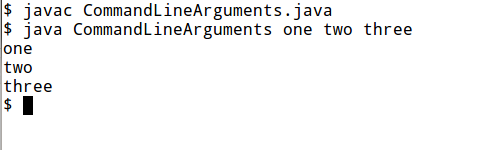
\includegraphics[scale=0.5]{CommandLineArguments.png}
 \end{center}
 \end{figure}

\subsection*{Passing Numeric CommandLine Arguments}
If an application needs to support a numeric command line argument, it must convert a String argument that represents a number, such as ``34'', to a numeric value. 

Here is a code snippet that converts a command-line argument to an \lstinline!int!.

\lstinputlisting{../Code/CommandLineNumArg.java}
\begin{figure}[H]
 \begin{center}
   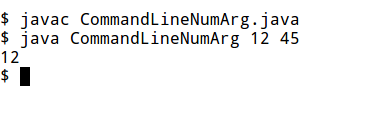
\includegraphics[scale=0.5]{CommandLineNumArg.png}
 \end{center}
 \end{figure}

\texttt{parseInt} throws a \texttt{NumberFormatException} if the format of \texttt{args[0]} is not valid. All of the \texttt{Number} classes \texttt{Integer}, \texttt{Float}, \texttt{Double}, and so on have \texttt{parseXXX} methods that convert a \texttt{String} representing a number to an object of their type.

\subsection*{Important Points}
\begin{itemize}
\item Command Line Arguments can be used to specify configuration information while launching your application.
\item There is no restriction on the number of command line arguments. You can specify any number of arguments.
\item Information is passed as Strings.
\item They are captured into the String argument of your main method.
\end{itemize}
\section*{String class}
Generally, string is a sequence of characters. But in java, string is an object that represents a sequence of characters. \texttt{String} class is used to create string object. The java \texttt{String} is immutable i.e. it cannot be changed but a new instance is created. For mutable class, you can use \texttt{StringBuffer} and \texttt{StringBuilder} class.

We will discuss about immutable string later. Let's first understand what is string in java and how to create the string object

Java String is, however, special. Unlike an ordinary class
 \begin{itemize}
  \item String is associated with string literal in the form of double-quoted text such as ``Hello world''. You can assign a string literal directly into a String variable, instead of calling the constructor to create a String instance.
\item The `+' operator is overloaded to concatenate two String operands. `+' does not work on any other objects.
\item String is immutable. That is, its content cannot be modified once it is created. 

String s = ``abc'';

String s2 = ``abc'';

Memory for \texttt{s} and \texttt{s2} are allocated as below.
\vfill{\ }
\begin{figure}[H]
 \begin{center}
   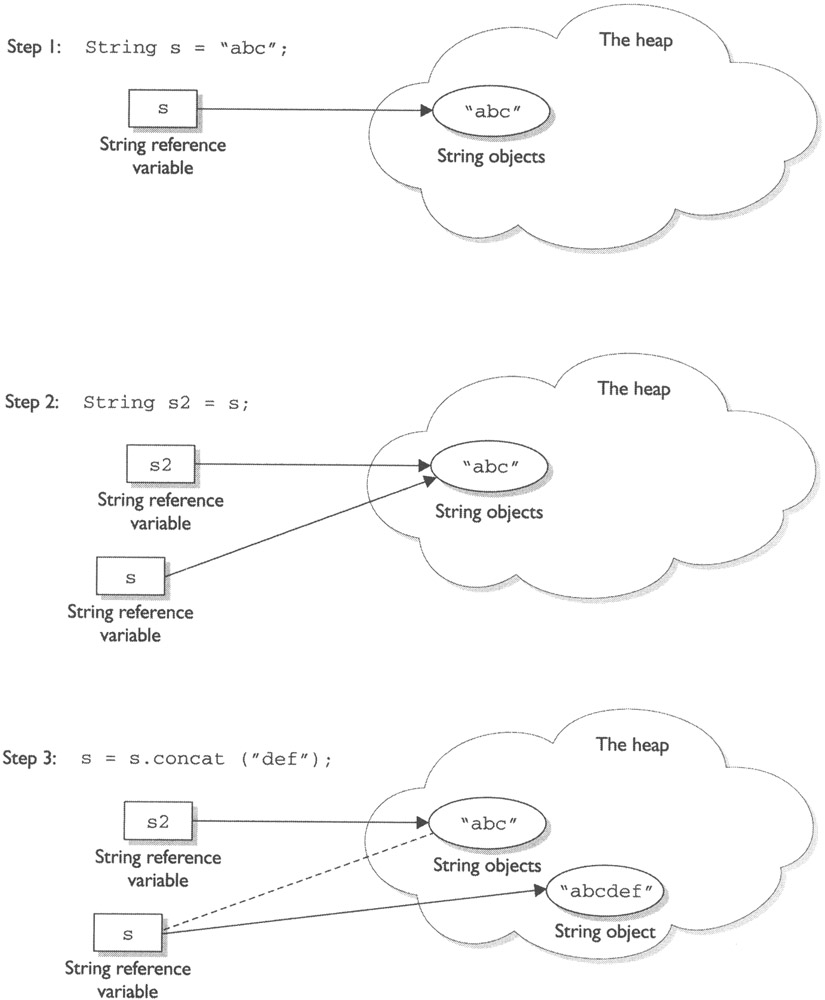
\includegraphics[scale=.4]{string.jpg}
\caption{String objects}
  \end{center}
 \end{figure}
 \end{itemize}

\subsubsection*{Creating a String object}
String objects can be created in two ways.
\begin{description}
\item [String Literal]

is a simple string enclosed in double quotes (`` ''). A string literal is treated as a String object.
 \begin{lstlisting}[numbers=none]
String str = ``Talentsprint'';
\end{lstlisting}

\item [new operator] creates an instance of String class.

 \begin{lstlisting}[numbers=none]
String str = new String(``Java'');
\end{lstlisting}

\end{description}
\begin{figure}[H]
 \begin{center}
   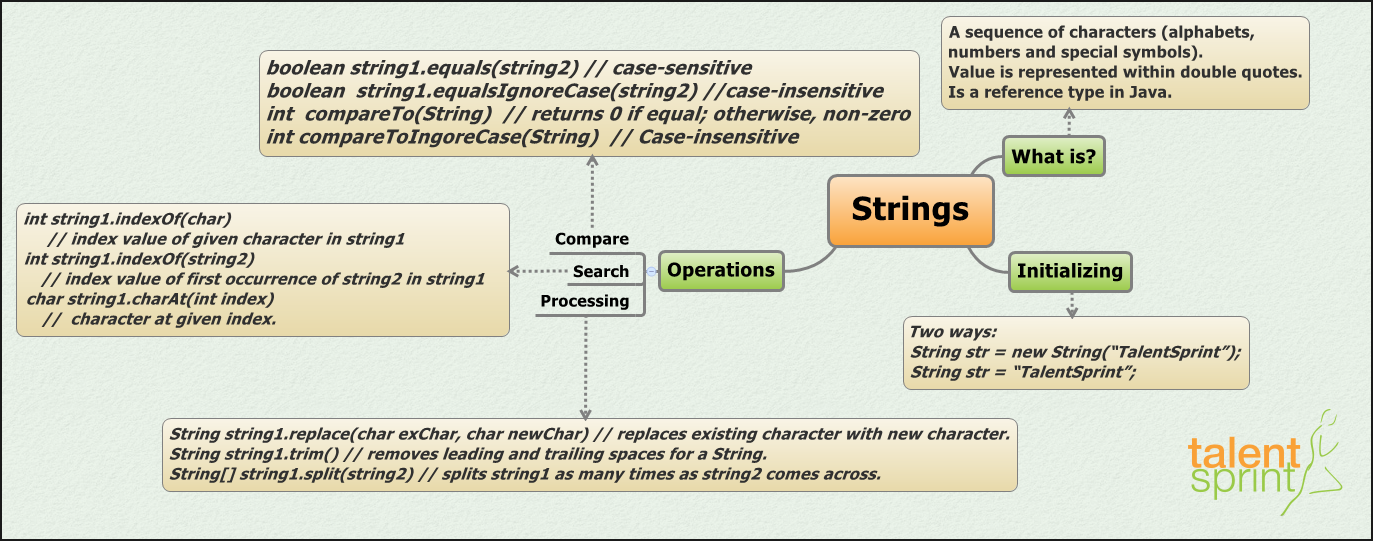
\includegraphics[angle=90,height=19cm, width=12cm]{Strings_Basics.png}
  
 \end{center}
 \end{figure}
\subsubsection*{String Class Methods}
\begin{description}
\item [charAt(int index)] returns the \texttt{character} at the specified index.

\begin{itemize}
\item \lstinline!char charAt(int index);!
\end{itemize}

\item [compareTo(String anotherString)] compares two strings lexicographically, based on the Unicode value of each character in the Strings.

\begin{itemize}
\item \lstinline!int compareTo(String anotherString);!
\end{itemize}
\item [compareToIgnoreCase(String str)] compares two strings lexicographically, ignoring case differences.

\begin{itemize}
\item \lstinline!int compareToIgnoreCase(String str);!
\end{itemize}
\item [concat(String str)] concatenates the specified string to the end of this string.

\begin{itemize}
\item \lstinline!String concat(String str);!
\end{itemize}
\item [equals(Object anObject)] compares this string to the specified object.

\begin{itemize}
\item \lstinline!boolean equals(Object anObject);!
\end{itemize}
\item [equalsIgnoreCase(String anotherString)] compares this String to another String, ignoring case considerations.

\begin{itemize}
\item \lstinline!String equalsIgnoreCase(String anotherString);!
\end{itemize}
\item [length()] returns the number of Unicode characters contained in the String.

\begin{itemize}
\item \lstinline!int length();!
\end{itemize}
\item [replace(char oldChar, char newChar)] returns a new string resulting from replacing all occurrences of \texttt{oldChar} in this string with \texttt{newChar}.

\begin{itemize}
\item \lstinline!String replace(char oldChar, char newChar);!
\end{itemize}
\item [substring(int beginIndex, int endIndex)] returns the substring of this string starting at the specified \texttt{beginIndex} up to the \texttt{endIndex} index.

\begin{itemize}
\item \lstinline!String substring(int beginIndex, int endIndex);!
\end{itemize}
\item [trim()] returns a copy of the string, with leading and trailing whitespace omitted.

\begin{itemize}
\item \lstinline!String trim();!
\end{itemize}



\end{description}
\vfill{\ }
\begin{figure}[H]
 \begin{center}
   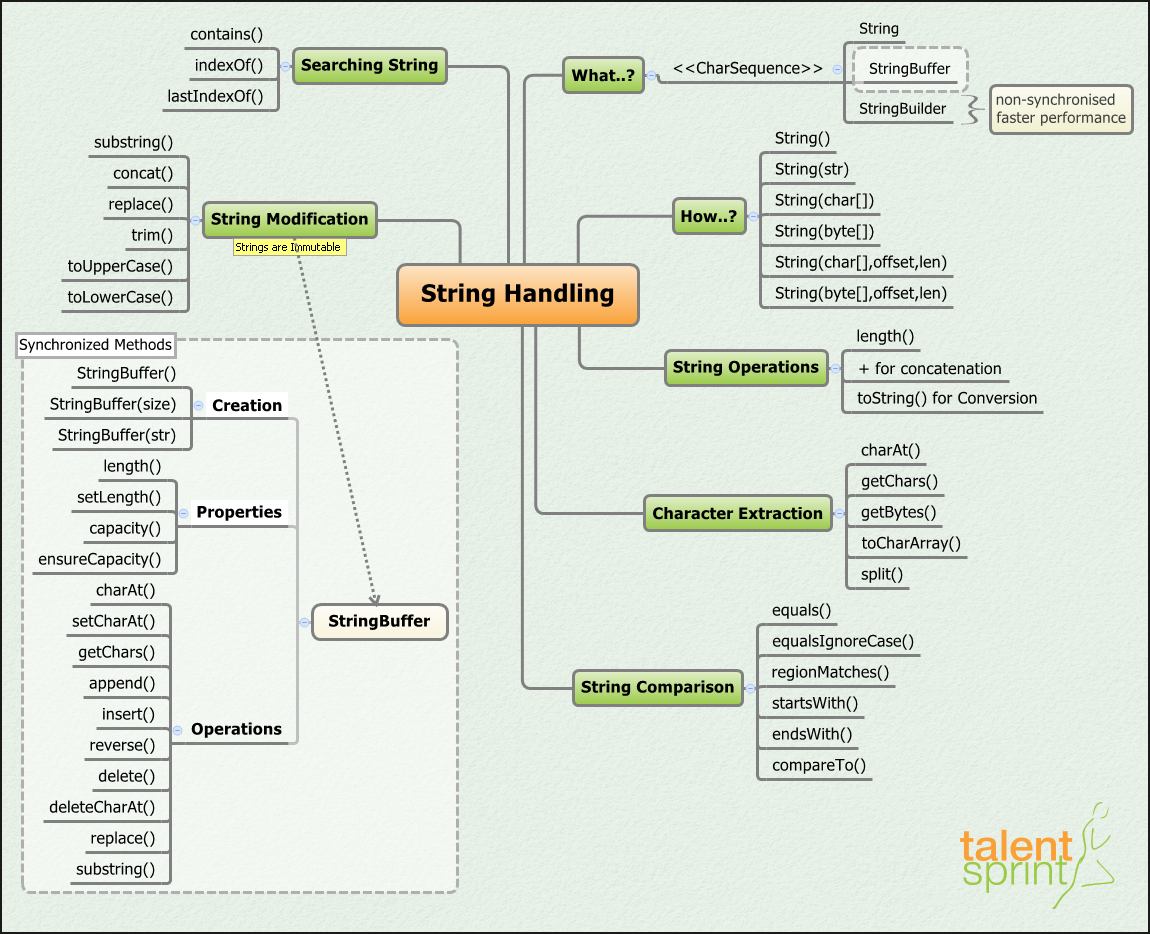
\includegraphics[angle=90,height=18cm, width=12cm]{StringHandling.png}
   
 \end{center}
 \end{figure}
\section*{StringBuffer and StringBuilder}
\subsection*{StringBuffer class}
The StringBuffer class is used to created mutable (modifiable) string. The StringBuffer class is same as String except it is mutable i.e. it can be changed.

Strings that need modification are handeled by \lstinline!StringBuffer! class After creating a \lstinline!StringBuffer!, new string(s) can be inserted or appendedto it. The size of \lstinline!StringBuffer! can change whenever needed. \lstinline!StringBuffer! objects can be dynamically altered. When a \lstinline!StringBuffer! is created, space for 16 more characters is always appened to it. This helps the \lstinline!StringBuffer! object to grow by 16 characters without any other process. When the string grows beyound the free 16 character space, \lstinline!StringBuffer! is relocated to a new memory space with required size.

\subsubsection*{StringBuffer Class Methods}
\begin{description}
\item [append(String s)] is used to append the specified string with this string. The \texttt{append()} method is overloaded like \texttt{append(char)}, \texttt{append(boolean)}, \texttt{append(int)}, \texttt{append(float)}, \texttt{append(double)} etc.

\begin{itemize}
\item \lstinline!StringBuffer append(String s);!
\end{itemize}
\item [insert(int offset, String s)]  is used to insert the specified string with this string at the specified position. The \texttt{insert()} method is overloaded like \texttt{insert(int, char), insert(int, boolean), insert(int, int), insert(int, float), insert(int, double)} etc.

\begin{itemize}
\item \lstinline!StringBuffer insert(int offset, String s);!
\end{itemize}
\item [delete(int startIndex, int endIndex)]  is used to delete the string from specified \texttt{startIndex} and \texttt{endIndex}.

\begin{itemize}
\item \lstinline!StringBuffer delete(int startIndex, int endIndex);!
\end{itemize}
\item [reverse()] is used to reverse the string.

\begin{itemize}
\item \lstinline!String reverse();!
\end{itemize}
\item [toString()]  returns a string representing the data in this sequence.

\begin{itemize}
\item \lstinline!String toString();!
\end{itemize}
\end{description}
\subsection*{StringBuilder}
JDK 1.5 introduced a new StringBuilder class (in package java.lang), which is almost identical to the StringBuffer class, except that it is not synchronized.

StringBuilder API-compatible with the StringBuffer class, i.e., having the same set of constructors and methods, but with no guarantee of synchronization. It can be a drop-in replacement for StringBuffer under a single-thread environment.


\end{document}
